\documentclass[../../../main_math.tex]{subfiles}

\begin{document}
\renewcommand{\col}{\geo}
\begin{multicols}{2}[\section{Algebraic topology}]

  	\subsection{Homotopy and fundamental group}
  	\subsubsection{Homotopy between maps and spaces}
  	
  	\begin{definition}
	  	Let $X,Y$ be two topological spaces \footnote{From now on $X$, $Y$ and $Z$ will always be topological spaces} and let $f,g: X \to Y$ be two continuous maps. A \emph{homotopy} between $f$ and $g$ is a continuous map $H:X\times [0,1] \to Y$ such that for all $x\in X$
	  	\begin{enumerate}
		  		\item $H(x,0)=f(x)$
		  		\item $H(x,1)=g(x)$.
		\end{enumerate}
		We say that $f$ and $g$ are \emph{homotopic} if there exists a homotopy between them, and we denote it by $f\simeq g$.
	\end{definition}
	  
	\begin{lemma}
	    Let $X=A\cup B$, where $A$ and $B$ are closed sets. If $\varphi: A \to Y$ and $\psi: B \to Y$ are continuous maps such that $\left.\varphi \right|_{A\cap B}=\left.\psi \right|_{A\cap B}$, then the map $$x\mapsto \begin{cases}
	    	\varphi(x) & \quad\text{if  } x\in A \\
	    	\psi(x)  & \quad\text{otherwise}\\
		\end{cases}$$ is also continuous.
	\end{lemma}
	
	\begin{proposition}
		The relation $\simeq$ is an equivalence relation between continuous maps.
    \end{proposition}
		
	\begin{definition}
		A continuous map $f:X\to Y$ is called a \emph{homotopy equivalence} if there exists a map $g:Y\to X$ such that $f\circ g\simeq id_Y$ and $g\circ f \simeq id_X$. We say that $X$ and $Y$ are \emph{homotopy equivalent} or that they have the same \emph{type of homotopy} if there exists a homotopy equivalence between them, and we denote it by $X\simeq Y$.
	\end{definition}

  	\begin{proposition}
		The relation $\simeq$ is an equivalence relation between topological spaces.
	\end{proposition}

	\begin{definition}
		A space having the homotopy type of a point is called \emph{contractible}.
	\end{definition}
	
	\subsubsection{Paths and foundamental group}
	
	\begin{definition}
		A \emph{path} in $X$ is a continuous map $\sigma:[0,1]\to X$.
	\end{definition}

	\begin{definition}
		Let $\sigma, \tau : [0,1]\to X$ be two paths such that $\sigma(0)=\tau(0)$ and $\sigma(1)=\tau(1)$. A homotopy between them is a continuous map $H:[0,1]\times [0,1] \to X$ such that
		\begin{enumerate}
			\item $H(s,0)=\sigma(s) $ $\forall s\in [0,1]$
			\item $H(s,1)=\tau(s)$ $\forall s\in [0,1]$
			\item $H(0,t)=\sigma(0)=\tau(0)$ $\forall t\in [0,1]$
			\item $H(1,t)=\sigma(1)=\tau(1)$ $\forall t\in [0,1]$
		\end{enumerate}
	When there exists a homotopy between $\sigma$ and $\tau$ we say that they are \emph{homotopic}, and we write $\sigma \simeq \tau $.
	\end{definition}

	\begin{proposition}
		The relation $\simeq$ is an equivalence relation between paths.
	\end{proposition}

	\begin{definition}
		Let $\sigma, \tau: [0,1] \to X$ such that $\sigma(1)=\tau(0)$. We define the product of $\sigma, \tau$ as 
		\begin{align*}
			\sigma \cdot \tau: [0,1] &\longrightarrow X \\
			x&\longmapsto \begin{cases}
				\sigma(2s) & 0\leq s \leq \frac{1}{2}\\
				\tau(2s-1)  & \frac{1}{2}\leq s \leq 1\\
			\end{cases}.
		\end{align*}
	
	\end{definition}

	\begin{lemma}\label{ProdCamins}
		Let $\sigma, \sigma', \tau, \tau':[0,1]\to X$ be paths such that 
		
		\begin{minipage}{0.29\textwidth}
			
			\begin{enumerate}
				\item $\sigma(0)=\sigma'(0)$
				\item $\sigma(1)=\sigma'(1)=\tau(0)=\tau'(0)$
				\item $\tau(1)=\tau'(1)$.
			\end{enumerate}
		\end{minipage}
		\begin{minipage}{0.21\textwidth}
			\begin{flushright}
				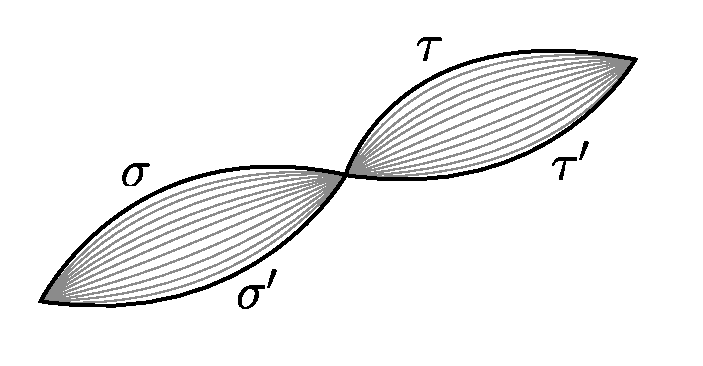
\includegraphics[width=0.9\textwidth]{Images/Camins.pdf}
			\end{flushright}
		\end{minipage}
	
	\vspace{0.1cm}
	If $\sigma \simeq \sigma'$ and $\tau \simeq \tau'$ then $\sigma \cdot \tau \simeq \sigma' \cdot \tau'$.
	\end{lemma}
	
	\begin{definition}
		A \emph{loop at the basepoint $x_0$} is a path $\sigma: [0,1]\to X$ such that $\sigma(0)=\sigma(1)=x_0$.
	\end{definition}

	\begin{definition}
		The \emph{foundamental group} of $X$ at the basepoint $x_0$ is the set of all homotopy classes of loops at the basepoint $x_0$, and it is denoted by $\pi_1 (X,x_0)$. We define $[\sigma]\cdot [\tau]:=[\sigma \cdot \tau]$, which is well-defined by \cref{ProdCamins}.
	\end{definition}

	\begin{proposition}
		$\big(\pi_1(X,x_0), \cdot \big)$ is a group.
	\end{proposition}
	
	\begin{proposition}
		Let $x_0, y_0 \in X$. If there exists a path $\gamma: [0,1] \to X$ from $x_0$ to $y_0$ then $\pi_1 (X,x_0) \cong \pi_1 (X,y_0)$.
	\end{proposition}
	
	\begin{proof}
		\begin{align*}
			\varphi: \pi_1(X,x_0) &\longrightarrow \pi_1(X,y_0) \\
			[\sigma]&\longmapsto [\gamma \cdot \sigma \cdot \gamma^{-1}]\\
		\end{align*}
		is an isomorphism.
	\end{proof}
	
	\begin{definition}
		Let $f:X\to Y$ be a continuous map, and $x_0 \in X$. We define 
		\begin{align*}
			f_*: \pi_1 (X,x_0) & \longrightarrow \pi_1 (Y,f(x_0)) \\
			[\alpha] &\longmapsto [f\circ \alpha].
		\end{align*}
		
	\end{definition}

	\begin{proposition}
		Let $f,g:X\to Y$ and $h:Y \to Z $ be continuous maps. Then
		\begin{enumerate}
			\item $f_*$ is well-defined and it is a group homomorphism.
			\item If $f\simeq g$ and $f(x_0)=g(x_0)$, then $f_*=g_*$.
			\item $(h\circ f)_*=h_*\circ f_*$.
		\end{enumerate}
	\end{proposition}

	\begin{corollary}
		$X\simeq Y \implies \pi_1 (X,x_0) \cong \pi_1 (Y,f(x_0))$.
	\end{corollary}

	%EXPLICAR RELACIO ENTRE HOMOTOPIES I GRUPS AMB DIAGRAMES


	\subsubsection{Foundamental group of $S^1$}
	
	\begin{lemma}
		Let (X,d) be a compact metric space, and $\{U_1, ..., U_n\}$ a finite cover of open sets of $X$. Then there exists $\varepsilon>0$ such that $\forall x \in X$, $B(x,\varepsilon)\subset U_i$ for some $i$. Such a number $\varepsilon$ is called a Lebesgue number of the cover.
	\end{lemma}

	\begin{proof}
		Let $C_i=X\setminus U_i$.  Then the map 
		
		\begin{align*}			
			f:X &\longrightarrow [0, +\infty) \\
			x &\longmapsto \frac{1}{n} \sum d(x,C_i)			
		\end{align*}
		
		is a continuous map on a compact set and therefore reaches the minimum at $X$. The number $\varepsilon=\min f$ satisfies the desired properties.
	\end{proof}
	
	\begin{lemma}
		Let $\sigma: [0,1] \to S^1$ be a loop such that $\sigma(0)=(1,0)$. Then, there is a unique path $\tilde{\sigma}: [0,1] \to \mathbb{R}$ such that $\tilde{\sigma}(0)=0$ and $\operatorname{exp}\circ\,\tilde{\sigma}=\sigma$, where $\operatorname{exp}(x)=\exp{2\pi x i}$. Such a path $\tilde{\sigma}$ is called a \emph{lift} of $\sigma$. Morover, if $\sigma \simeq \tau$ then $\tilde{\sigma}(1)=\tilde{\tau}(1)$, and $\tilde{\sigma}(1)$ is called the degree of $\sigma$.
	\end{lemma}
	\begin{proof}
		Let $U=S^1\setminus\{(1,0)\}$ and $V=S^1\setminus\{(-1,0)\}$. Let $k\in \mathbb{N}$ be such that $1/k<\varepsilon$, where $\varepsilon$ is a Lebesgue number of the cover $\{\sigma^{-1}(U), \sigma^{-1}(V)\}\subset [0,1]$. For every $n\in \mathbb{N}$ $\operatorname{exp}: (n,n+1)\to U$ and $\operatorname{exp}: (n-\frac{1}{2},n+\frac{1}{2})\to V$ are homeomorphisms and, therefore, for every $1\leq i \leq k$ there exists a unique $\tilde{\sigma}_i: [\frac{i-1}{k}, \frac{i}{k}]\to \mathbb{R}$ such that $\operatorname{exp}\circ\,\tilde{\sigma_i}=\sigma|_{[\frac{i-1}{k}, \frac{i}{k}]}$, and $\tilde{\sigma}_{i+1}(\frac{i}{k})=\tilde{\sigma}_i(\frac{i}{k})$ if $i\geq 1$ and $\tilde{\sigma}_{1}(0)=0$. Finally, for $t\in[\frac{i-1}{k}, \frac{i}{k}]$ we define $\tilde{\sigma}(t)=\tilde{\sigma}_i(t)$. Now let us suppose that $H:[0,1]\times[0,1]\to S^1$ is a homotopy between $\sigma$ and $\tau$. A very similar argument shows that there exists a continuous map $\tilde{H}:[0,1]\times[0,1]\to \mathbb{R}$ such that $\operatorname{exp}\circ\, \tilde{H}=H$. Thus, $t\mapsto \tilde{H}(1,t)$ is an integer-valued continuous map and, therefore, it is constant, which means that $\tilde{\sigma}(1)=\tilde{H}(1,0)=\tilde{H}(1,1)=\tilde{\tau}(1)$.
	\end{proof}
	
	\begin{theorem}
		The foundamental group of $S^1$ is isomorphic to $\mathbb{Z}$
	\end{theorem}
	
	\begin{proof}
		\begin{align*}
			\varphi: \pi_1(S^1, (1,0)) &\longrightarrow \mathbb{Z} \\
			[\sigma]&\longmapsto \text{deg}(\sigma) \\
		\end{align*}
		is a well-defined isomorphism.
	\end{proof}
	
	\begin{definition}
		Let $A\subseteq X$ be a subspace of $X$. A \emph{retraction} of $X$ onto $A$ is a continuous map $r: X \to A$ such that $r(a)=a$ for all $a\in A$. If such a retraction exists, $A$ is called a \emph{retract} of $X$. 
	\end{definition}

	\begin{corollary}\label{retraccio}
		$S^1\subseteq \mathbb{D}^2$ is not a retract of $\mathbb{D}^2$.
	\end{corollary}

	%PROVA AMB DIAGRAMES

	\begin{theorem}[Brower theorem]
		\label{Brower}
		Every continuous map $f:\mathbb{D}^2 \to \mathbb{D}^2$ has a fixed point. 
	\end{theorem}

	\begin{proof}
		
		\begin{minipage}{0.3\textwidth}
			If $f(x)\neq x$ for every $x\in \mathbb{D}^2$, then the map $r: \mathbb{D}^2 \to S^1$ defined by $r(x)$ being the intersection of the line passing through $x$ and $f(x)$ and $S^1$ closest to $x$ is a retraction of $\mathbb{D}^2$ to $S^1$, which contradicts \cref{retraccio}.
		\end{minipage}
		\begin{minipage}{0.2\textwidth}
			\begin{center}
				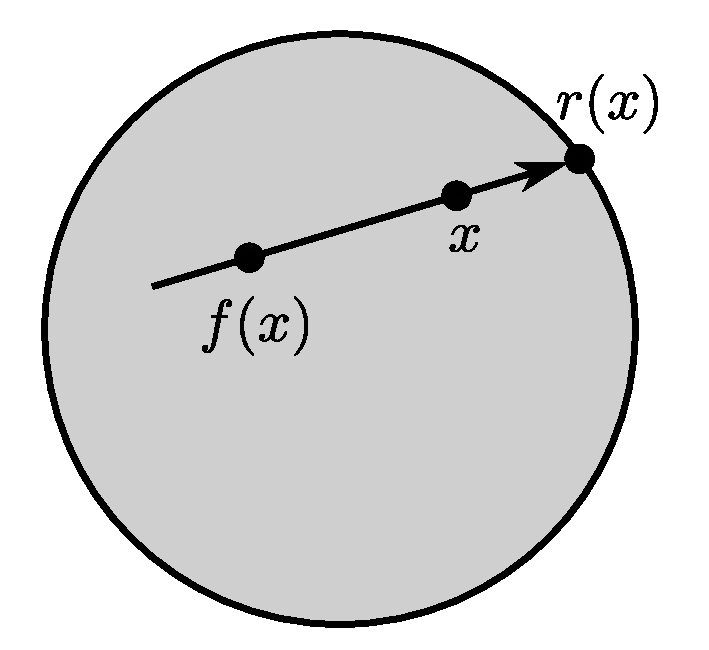
\includegraphics[width=0.6\textwidth]{Images/Brower.pdf}
			\end{center}
		\end{minipage}

	\end{proof}
	
	\begin{lemma} \label{lema Borsuk}
		Let $\alpha:[0,1]\to S^1$ be such that $\alpha(t+\frac{1}{2})=-\alpha(t)$ for all $t\in[0,\frac{1}{2}]$. Then, the degree of $\alpha$ is odd.
	\end{lemma}

	\begin{theorem}[Borsuk-Ulam theorem]
		\label{Borsuk-Ulam}
		If $f:S^2 \to \mathbb{R}^2$ is a continuous map, then there exists $x\in S^2$ such that $f(x)=f(-x)$.
	\end{theorem}
	
	\begin{proof}
		If $f(x)\neq f(-x)$ for all $x\in S^2$, then $g(x)=\frac{f(x)-f(-x)}{\|f(x)-f(-x)\|}$ is a continuous map from $S^2$ to $S^1$. Consider $h:[0,1] \to S^2$ defined by $h(t)=(\cos(2\pi t), \sin(2\pi t), 0)$, and $\alpha = g \circ h$. Then, since $h$ is contractile, $\alpha$ is also contractile, but $g(-x)=-g(x)\implies \alpha(t+1/2)=-\alpha(t)$, in contradiction with \cref{lema Borsuk}.
	\end{proof}
	
	\begin{corollary}
		Let $A_1, A_2, A_3\subseteq S^2$ be closed sets such that $S^2=A_1\cup A_2 \cup A_3$. Then there exists $x\in S^2$ such that $x,-x \in A_i$ for some $i$.
	\end{corollary}

	\begin{proof}
		Consider $f: S^2 \to \mathbb{R}^2$ such that $f(x)=(d_1(x), d_2(x))$, where $d_i(x)$ is the distance from $x$ to $A_i$, and apply \cref{Borsuk-Ulam}.
	\end{proof}
	
	\begin{proposition}
		$S^2$ is contractible.
	\end{proposition}
	
	\subsubsection{Seifert–Van Kampen theorem}
	\begin{definition}
		The \emph{free group} $F_S$ over a set $S$ is the set of all the finite words $s_1^{n_1}s_2^{n_2}...\,s_r^{n_r}$ such that $s_i \in S$, $n_i \in \mathbb{Z}\setminus\{0\}$ and $s_i \neq s_{i+1}$, and the empty word, which will the identity element. The group operation in $F_S$ is the juxtaposition, that is, 
		\begin{multline*}
			s_1^{n_1}...\,s_r^{n_r} \cdot g_1^{m_1}...\,g_r^{m_t}=\\
			= \begin{cases}
				s_1^{n_1}...\,s_r^{n_r}g_1^{m_1}...\,g_t^{m_t} & \quad\text{if  } s_r\neq g_1 \\
				s_1^{n_1}...\,s_r^{n_r+m_1}g_2^{m_2}...\,g_t^{m_t}  & \quad\text{if }s_r = g_1 \text{, } n_r+m_1 \neq 0\\
				s_1^{n_1}...\,s_{r-1}^{n_{r-1}}g_2^{m_2}...\,g_t^{m_t} & \quad\text{if }s_r = g_1 \text{, } n_r+m_1 = 0\\
			\end{cases}
		\end{multline*}
		
	\end{definition}

	
	\begin{proposition}
		Let $G$ be a group, and $S\subseteq G$ a generating set of $G$. Then, there exists an epimorphism from $F_S$ to G.
	\end{proposition}
	
	\begin{definition}
		Let $G$ be a group, $S\subseteq G$ a generating set of $G$, and $\varphi:F_S\to G$ an epimorphism. An element of $\ker(\varphi)$ is called a relation. If $R=\{r_i\}_{i\in I}$ is a set of relations such that $\triangleleft \, R \, \triangleright = \ker(\varphi)$, then we say that $G$ has a presentation $< S \, | \, R >$.
	\end{definition}

	\begin{definition}
		The free product $*_{i\in I}G_i$ of a set of groups $\{G_i\}_{i\in I}$ is the set of all finite words $g_1g_2...g_n$ such that $g_i\in G_{g_i}\setminus \{e_{g_i}\}$, where $e_{g_i}$ is the identity element of the group $G_{g_i}$.  The group operation in $*_{i\in I}G_i$ is the juxtaposition, that is, 
		\begin{multline*}
			g_1...\,g_r \cdot h_1...\,h_t=\\
			= \begin{cases}
				g_1...\,g_rh_1...\,h_t & \quad\text{if  } G_{g_r}\neq G_{h_1} \\
				g_1...\,(g_r\cdot h_1)h_2...\,h_t  & \quad\text{if } G_{g_r} = G_{h_1} \text{,  } g_r\cdot h_1 \neq e_{g_r}\\
				g_1...\,g_{r-1}h_2...\,h_t & \quad\text{if } G_{g_r} = G_{h_1} \text{,  } g_r\cdot h_1 = e_{g_r}\\
			\end{cases}
		\end{multline*}
	\end{definition}

	\begin{proposition}
		Let $\{G_i\}_{i\in I}$ be a set of groups, $G$ a group, and $f_i: G_i \to G$ a group homomorphism for every $i\in I$. Then, there exists a unique group homomorphism $\varphi: *_{i\in I}G_i \to G$ such that $\left.\varphi \right|_{G_i}=f_i$
	\end{proposition}

	\begin{theorem}[Seifert–Van Kampen theorem]
		If $X$ is the union of two path-connected open sets $U, V$ containing the basepoint $x_0$ such that $U\cap V$ is path-connected, then the homomorphism $\Phi : \pi_1(U, x_0)*\pi_1(V, x_0)\to \pi_1(X, x_0)$ defined by $\left.\Phi \right|_{\pi_1(U, x_0)}([\alpha]_U)=[\alpha]_X$ and  $\left.\Phi \right|_{\pi_1(V, x_0)}([\alpha]_V)=[\alpha]_X$ is surjective, and $\ker(\Phi)=\triangleleft\,\{[\alpha]_U[\alpha]_V^{-1} : [\alpha]_{U\cap V} \in \pi_1(U\cap V, x_0)\}\,\triangleright$.
	\end{theorem}

	\subsection{Singular Homology}
	
	\begin{definition}
		The standard $p$\emph{-simplex} is the set $$\Delta_p:=\{(x_0, ... , x_p)\in \mathbb{R}^{p+1}\ : x_i\geq0, \, \sum x_i =1\}$$
	\end{definition}
	
	\begin{definition}
		A \emph{singular $p$-simplex} (or simply \emph{$p$-simplex}) in $X$ is a continuous map $\sigma: \Delta_p \to X$.
	\end{definition}
	
	\begin{definition}
		We denote by $C_p(X)$ the abelian free group generated by the set of all $p$-simplex in $X$. An element of $C_p(X)$ is called a \emph{singular $p$-chain} (or simply a \emph{$p$-chain}). 
	\end{definition}

	\begin{definition}
		The $i$-th side of the standard $p$-simplex $\Delta_p$ is the $(p-1)$-simplex
		\begin{align*}
			F_i^p : \Delta_{p-1} &\longrightarrow \Delta_p \\
					(x_0, ..., x_{p-1}) & \longmapsto (x_0,...,x_{i-1}, 0, x_{i}, ..., x_{p-1}).
		\end{align*}
	\end{definition}

	\begin{definition}
		The $boundary$ of a $p$-simplex $\sigma$ is the $(p-1)$-chain $$\partial\sigma:= \sum_{i=0}^{p} (-1)^i \sigma \circ F_i^p,$$ and the boundary of a $p$-chain $\sum a_{\sigma} \sigma$ is the $(p-1)$-chain $$\partial \sum a_{\sigma} \sigma := \sum a_{\sigma} \partial\sigma.$$ 
	\end{definition}

	\begin{definition} 
		Let $c$ be a $p$-chain in $X$.
		\begin{enumerate}
			\item We say that a $c$ is a \emph{$p$-cycle} if $\partial c=0$. The set of all $p$-cycles in $X$ is denoted by $Z_p(X)$.
			\item We say that $c$ is a \emph{$p$-boundary} if there exists $c'\in C_{p+1}(X)$ such that $\partial c'=c$. The set of all \emph{$p$-boundarys} in $X$ is denoted by $B_p(X)$.
		\end{enumerate}
	\end{definition}

	\begin{proposition}
		$\partial : C_p \to C_{p-1}$ is a group homomorphism, and, therefore, $Z_p(X)$ and $B_p(X)$ are subgroups of $C_p(X)$.
	\end{proposition}
	
	\begin{lemma}
		Let $c$ be a $p$-chain. Then, $\partial \partial c=0$. As a result, $B_p(X)\subseteq Z_p(X)$.
	\end{lemma}

	\begin{definition}
		The $p$-th homology group of $X$ is $$H_p(X):=\quot{Z_p(X)}{B_p(X)}$$
	\end{definition}

	\subsubsection{Morphisms of chains}
	
	\begin{definition}
		Let $f: X \to Y$ be a continuous map. $f$ induces a map $f_{\#}$ from $C_p(X)$ to $C_p(Y)$ as follows:
		\begin{align*}
			f_{\#}: C_p(X) & \longrightarrow C_p(Y) \\
			\sum a_{\sigma} \sigma &\longmapsto \sum a_{\sigma} f\circ\sigma.
		\end{align*}
	
	\end{definition}

	\begin{proposition}\label{TAApInduida}
		Let $f:X\to Y$ be a continuous map. Then:
		\begin{enumerate}
			\item $f_{\#}$ is a group homomorphism.
			\item $f_{\#}\circ \partial= \partial \circ f_{\#}$.
			\item $f_{\#}(Z_p(X))\subseteq Z_p(Y)$, and $f_{\#}(B_p(X))\subseteq B_p(Y)$. Therefore, $f_{\#}$ induces a group homeomorphism $f_{*}: H_p(X) \to H_p(Y)$.
		\end{enumerate}
	\end{proposition}
	
	\begin{definition}
		Let $f: X \to Y$ be a continuous map. $f$ induces a group homomorphism $f_{*}$ from $H_p(X)$ to $H_p(Y)$ defined by $f_{*}([c])=[f_{\#}(c)]$, $c\in C_p(X)$, which is well-defined by \cref{TAApInduida}.
	\end{definition}
	
	\begin{proposition}
		Let $f:X\to Y$, $g:Y\to Z$ be two continuous maps. Then,
		\begin{enumerate}
			\item $(f\circ g)_{*}=g_{*}\circ f_{*}$.
			\item $(id_{X})_*=id_{H_p(X)}$.
		\end{enumerate}
	\end{proposition}

	\begin{corollary}
		If $f:X\to Y$ is an homeomorphism, then $f_*: H_p(X) \to H_p(Y)$ is a group isomorphism.
	\end{corollary}

	\begin{proposition}
		Let $X=\bigsqcup X_{\alpha}$ be the decomposition of $X$ in path-connected components, and $i_{\alpha}:X_{\alpha} \to X$ the inclusion. Then $\bigoplus_{\alpha} i_{\alpha}: \bigoplus_{\alpha} H_p(X_{\alpha}) \to H_p(X)$ is a group isomorphism.
	\end{proposition}
	
	\begin{proposition}
		If $X$ is path-connected, then $H_0(X)\cong \mathbb{Z}$.
	\end{proposition}

	\begin{proof}
		\begin{align*}
			\varepsilon: H_0(X)&\longrightarrow \mathbb{Z} \\
			\bigg[ \sum a_{\sigma}\sigma \bigg] &\longmapsto \sum a_{\sigma}
		\end{align*}
	is a well-defined group isomorphism.
	\end{proof}
	
	\subsubsection{Relationship between homotopy and homology}
	\begin{lemma}
		Let $f,g:X\to Y$ be two continuous maps such that $f\simeq g$. There exisits a group homomorphism $P: C_p(X)\to C_{p+1}(Y)$ such that $\partial P + P\partial =g_{\#}-f_{\#}$.
	\end{lemma}

	\begin{theorem}
		Let $f,g:X\to Y$ be two continuous maps. If $f\simeq g$, then $f_*=g_*$.
	\end{theorem}

	\begin{corollary}
		If $X\simeq Y$, then $H_p(X)\cong H_p(Y)$.
	\end{corollary}
 
\end{multicols}
\end{document}